\chapter{Energieversorgung}
\label{Energieversorgung}
% ================ Einstellungen =======================
\thispagestyle{fancy} \rhead{\slshape Energieversorgung}
% ======================================================

Wie in allen Bereichen des vorliegenden Projekts geht es auch im Bereich der Energieversorgung darum, aus dem verfügbaren Raum, kosteneffizient eine möglichst gute Performance zu erhalten. Um dies zu erreichen, muss der Energiebedarf der Elektronik auf ein Minimum reduziert werden. Mit der Auswahl von energieeffizienten Komponenten und einem effizienten Ablauf im Programmcode, kann dem Energieverbrauch entgegengewirkt werden. Der Energiebedarf von Komponenten, die gerade nicht in Verwendung sind, kann so erheblich reduziert werden. Wird zum Beispiel der Mikrocontroller nicht aktiv verwendet, versetzt er sich in einen sparsamen Bereitschaftsmodus, der einen wesentlich geringeren Verbrauch hat.

\section{Technische Grundlagen}
 
Die maximale Grösse des Akkus war durch das designte Gehäuse bereits vorgegeben. Somit konnte eine einfache Auswahl getroffen werden. Um den Energiebedarf des Dojos abzuschätzen, wurde zu Beginn der Projektarbeit eine Energiebedarfsberechnung anhand von Datenblattangaben der verwendeten Komponenten gemacht. Die Berechnungen haben gezeigt, dass das Wunschziel, die Akkulaufzeit des Dojos auf einen ganzen Museumstag auszulegen, ins Auge gefasst werden kann. Dies führt im Museum zu einer hohen Verfügbarkeit der Geräte.  Das Museum benötigt so wesentlich weniger Geräte und muss nicht ständig die Geräte auswechseln und aufladen. Ausserdem verringert sich der Arbeitsaufwand, da die Dojos nicht in jeder freien Minute ins Ladegerät gesteckt werden müssen, sondern ein Ladezyklus über Nacht ausreicht.\\

Die ursprüngliche Energiebedarfsberechnung der wichtigsten Komponenten hat bei einer durchschnittlichen Nutzung von zehn Stunden einen Speicherbedarf von $400mAh$ ergeben. Es wurde angenommen, dass das Dojo während einem Drittel der Zeit aktiv genutzt und in der übrigen Zeit in Standby-Modus versetzt wird.\\ 

 
\section{Akku, Ladesteuerung und Spannungsregelung}

Aufgrund der Voraussetzungen wurde bei der Suche auf Akkus des Typen LI14500 fokussiert, Lithium-Akkus mit einem Durchmesser von $14mm$ und einer Länge von $50mm$. Diese Standardgrösse ist für das vorgegebene Gehäuse etwas zu gross, weshalb es etwas angepasst werden muss. Die Grösse solcher Akkus mit den Anforderungen der Energiekapazität sind auf dem Markt auffindbar.\\

Das Dojo wird über den integrierten USB-Anschluss aufgeladen. Die Ladesteuerung ist Aufgabe des MCP7383 von Microchip . Dieser Ladesteuerungs-IC benötigt wenige zusätzliche Bauteile und ist daher ideal für portable Geräte wie das Dojo geeignet, er arbeitet nach dem Prinzip constand-current / constant-voltage. Die Ladeschaltung ist auf der Hauptplatine integriert. Die verwendete Standardbeschaltung ist auf Abbildung \ref{fig:Ladeschaltung} ersichtlich, die Ladekurve ist in Abbildung \ref{fig:Ladekurve} dargestellt. In der Ladekurve ist gut zu erkennen, wie die Spannung gegen Ende der Ladung konstant gehalten und der Strom reduziert wird.\\

%%%%%%
\begin{figure}[htp]
	\centering
	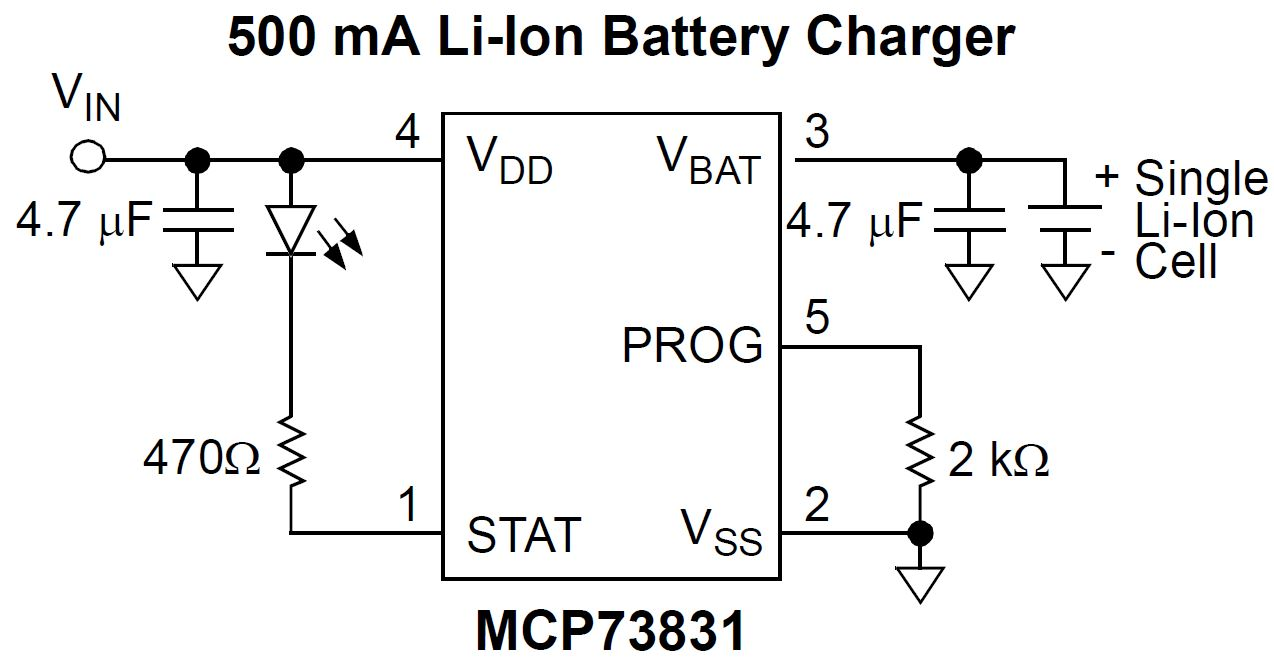
\includegraphics[width=10cm]{Bilder/LadeschaltungSchema.JPG}
	 \caption{Schema der Ladeschaltung}
	 \label{fig:Ladeschaltung}
\end{figure}
%%%%%%

%%%%%%
\begin{figure}[htp]
	\centering
	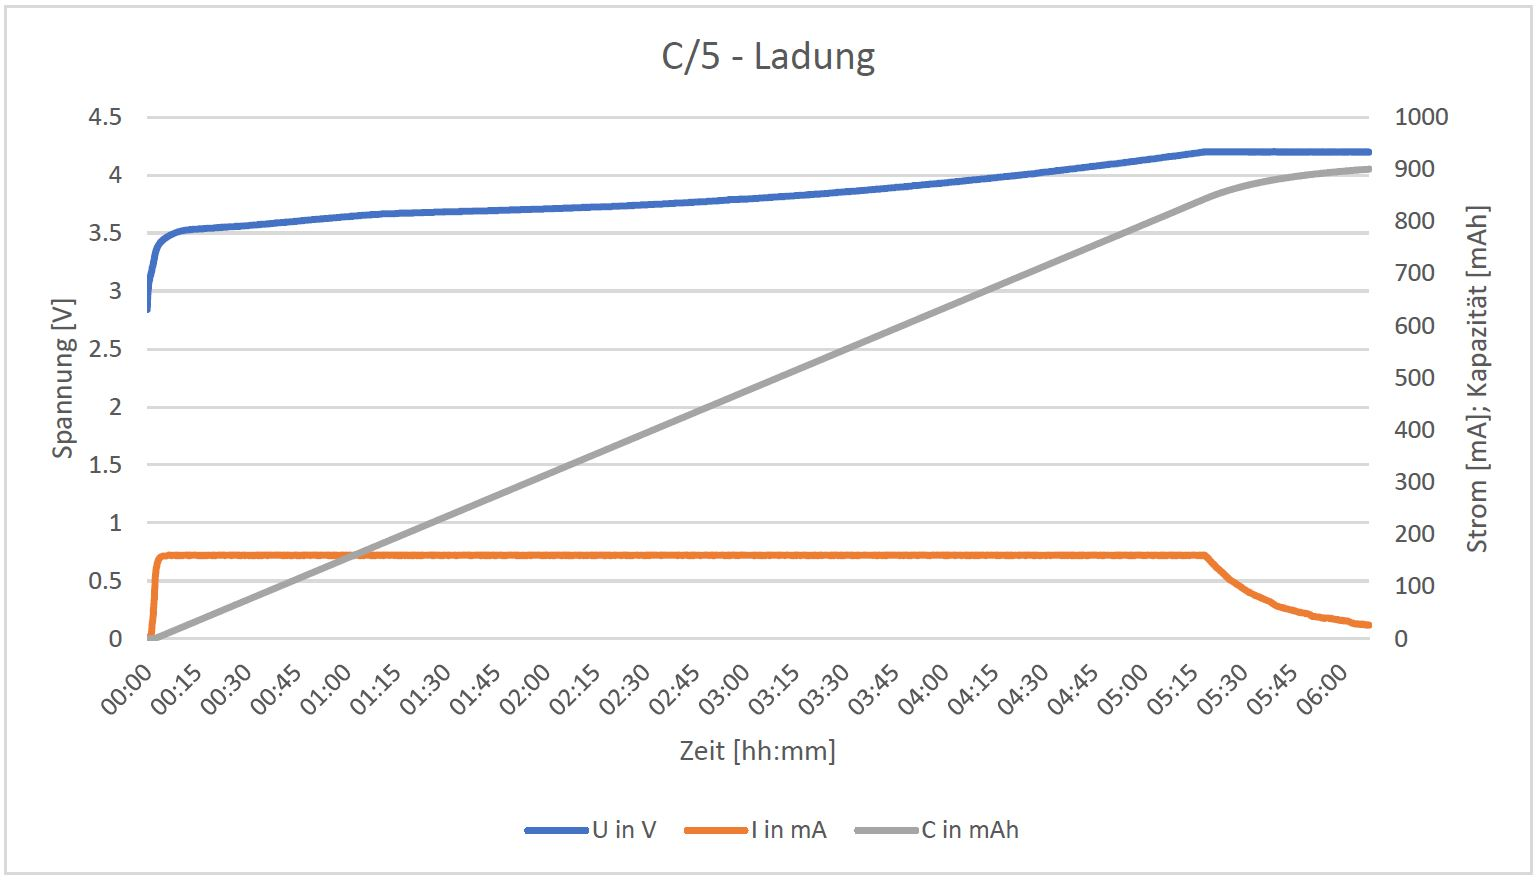
\includegraphics[width=15cm]{Bilder/Ladekurve.JPG}
	 \caption{Ladekurve des Emmerich-Akkus}
	 \label{fig:Ladekurve}
\end{figure}
%%%%%%

%-> Ladekurve (und entsprechende Referenzierung) evtl. wieder entfernen. Ist an dieser Stelle eigentlich sowieso nicht ganz korrekt, die Entladekurve wurde nämlich nicht zusammen mit dem Print und der entsprechenden Ladeschaltung auf dem Print generiert, sondern nur mit dem Akku direkt am Akkulade-/Entladegerät...

Um die interne Spannungsversorgung auf einem konstanten Niveau zu halten, ist dem Akku der LDO (Low Drop-Out) TC1262 von Microchip nachgeschaltet. Dieser regelt die Betriebsspannung auf $3.3V$, liefert bis zu $500mA$ und ist selbst sehr energiesparend.


\section{Validierung}

Nach Empfang des Emmerich-Akkus konnte dieser erfolgreich mit dem angefertigten Prototyp des Dojo-Prints in Betrieb genommen werden. Um die tatsächliche Kapazität des Akkus zu bestimmen und um zu verifizieren, ob die Lieferantenangabe stimmt, wurde der Akku in verschiedenen Durchläufen getestet. Die Tests wurden mit dem ``Battery Charging Centre ALC 8500-2 Expert'' von der ELV Elektronik AG durchgeführt (Abbildung \ref{fig:ALCExpert}). Zu diesem Testgerät gibt es eine PC-Software (Abbildung \ref{fig:ChargeProfessional}), mit der Parameter wie die Art des Akkus, Kapazität, Spannung aber auch das gewünschte Lade- / Entladeprofil eingestellt werden können. Während dem Vorgang, also dem Laden oder Entladen des Akkus, speichert das Gerät alle fünf Sekunden die Werte der aktuellen Spannung, des aktuellen Stromes sowie der summierten Kapazität in mAh. Anschliessend können die abgespeicherten Werte zur weiteren Auswertung über die PC-Software in eine Tabelle exportiert werden.\\

%%%%%%
\begin{figure}[htp]
	\centering
	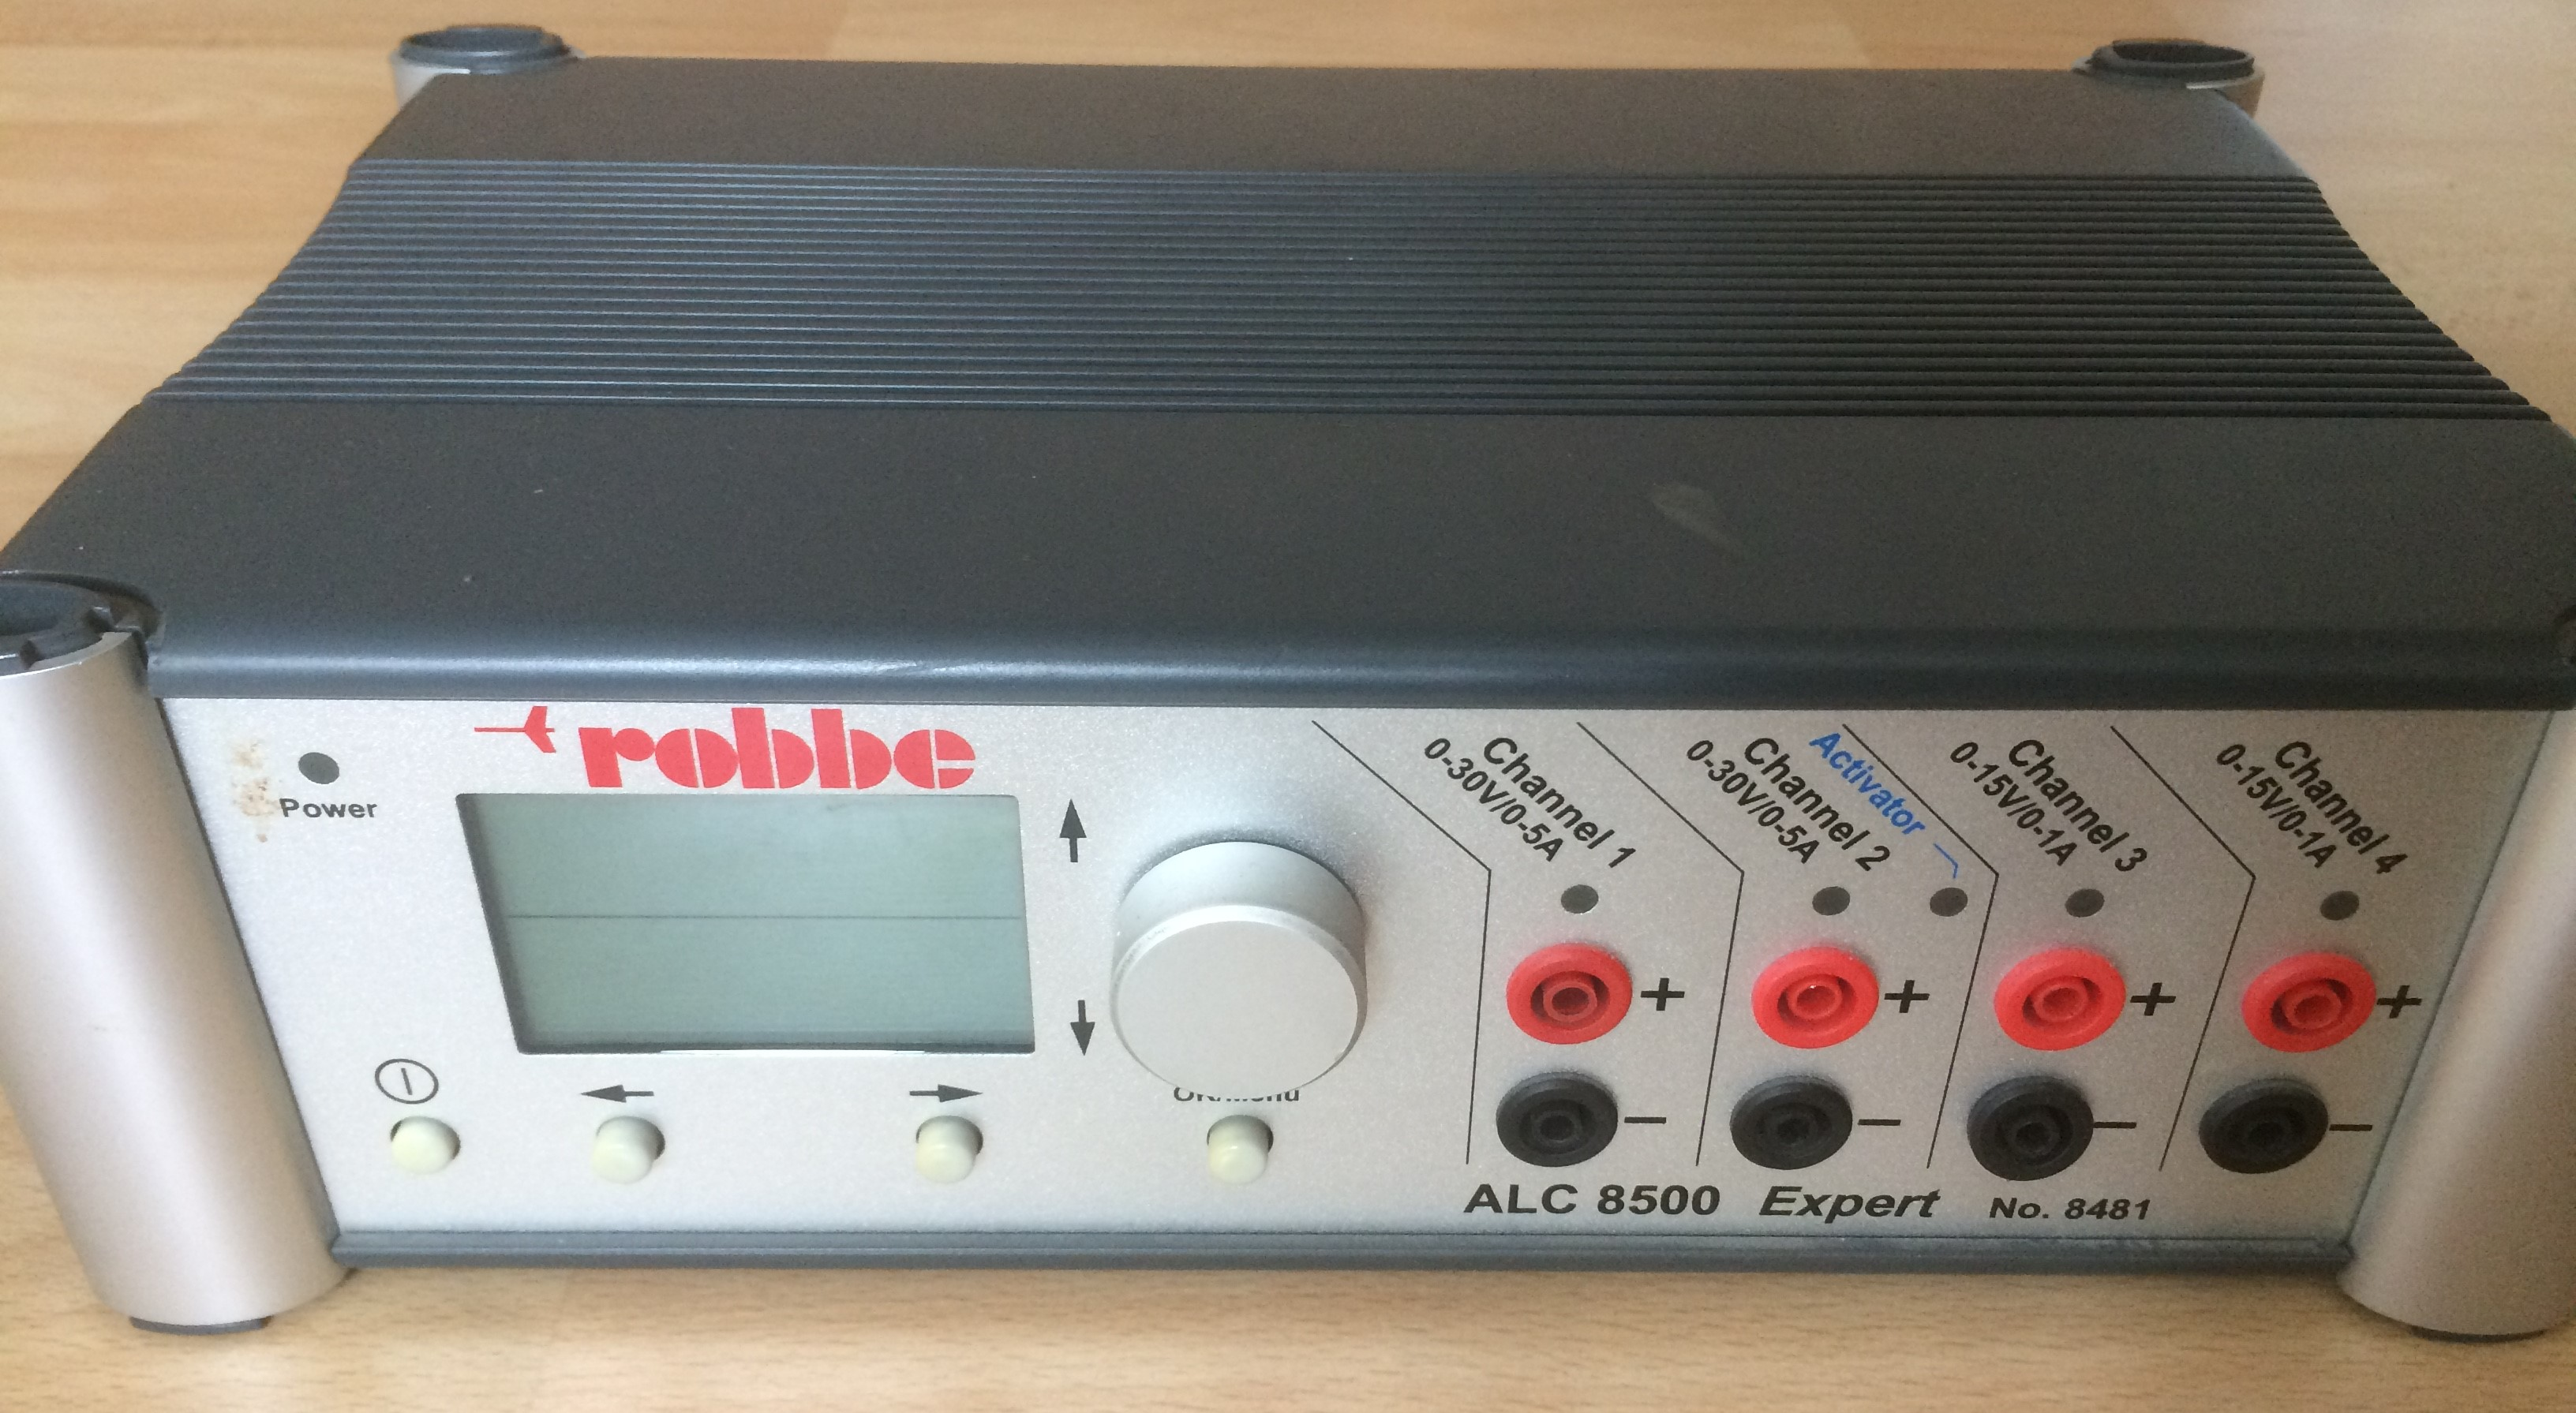
\includegraphics[width=7cm]{Bilder/ALC8500Expert.JPG}
	 \caption{Das verwendete Akkutestgerät ALC 8500 Expert}
	 \label{fig:ALCExpert}
\end{figure}
%%%%%%

%%%%%%
\begin{figure}[htp]
	\centering
	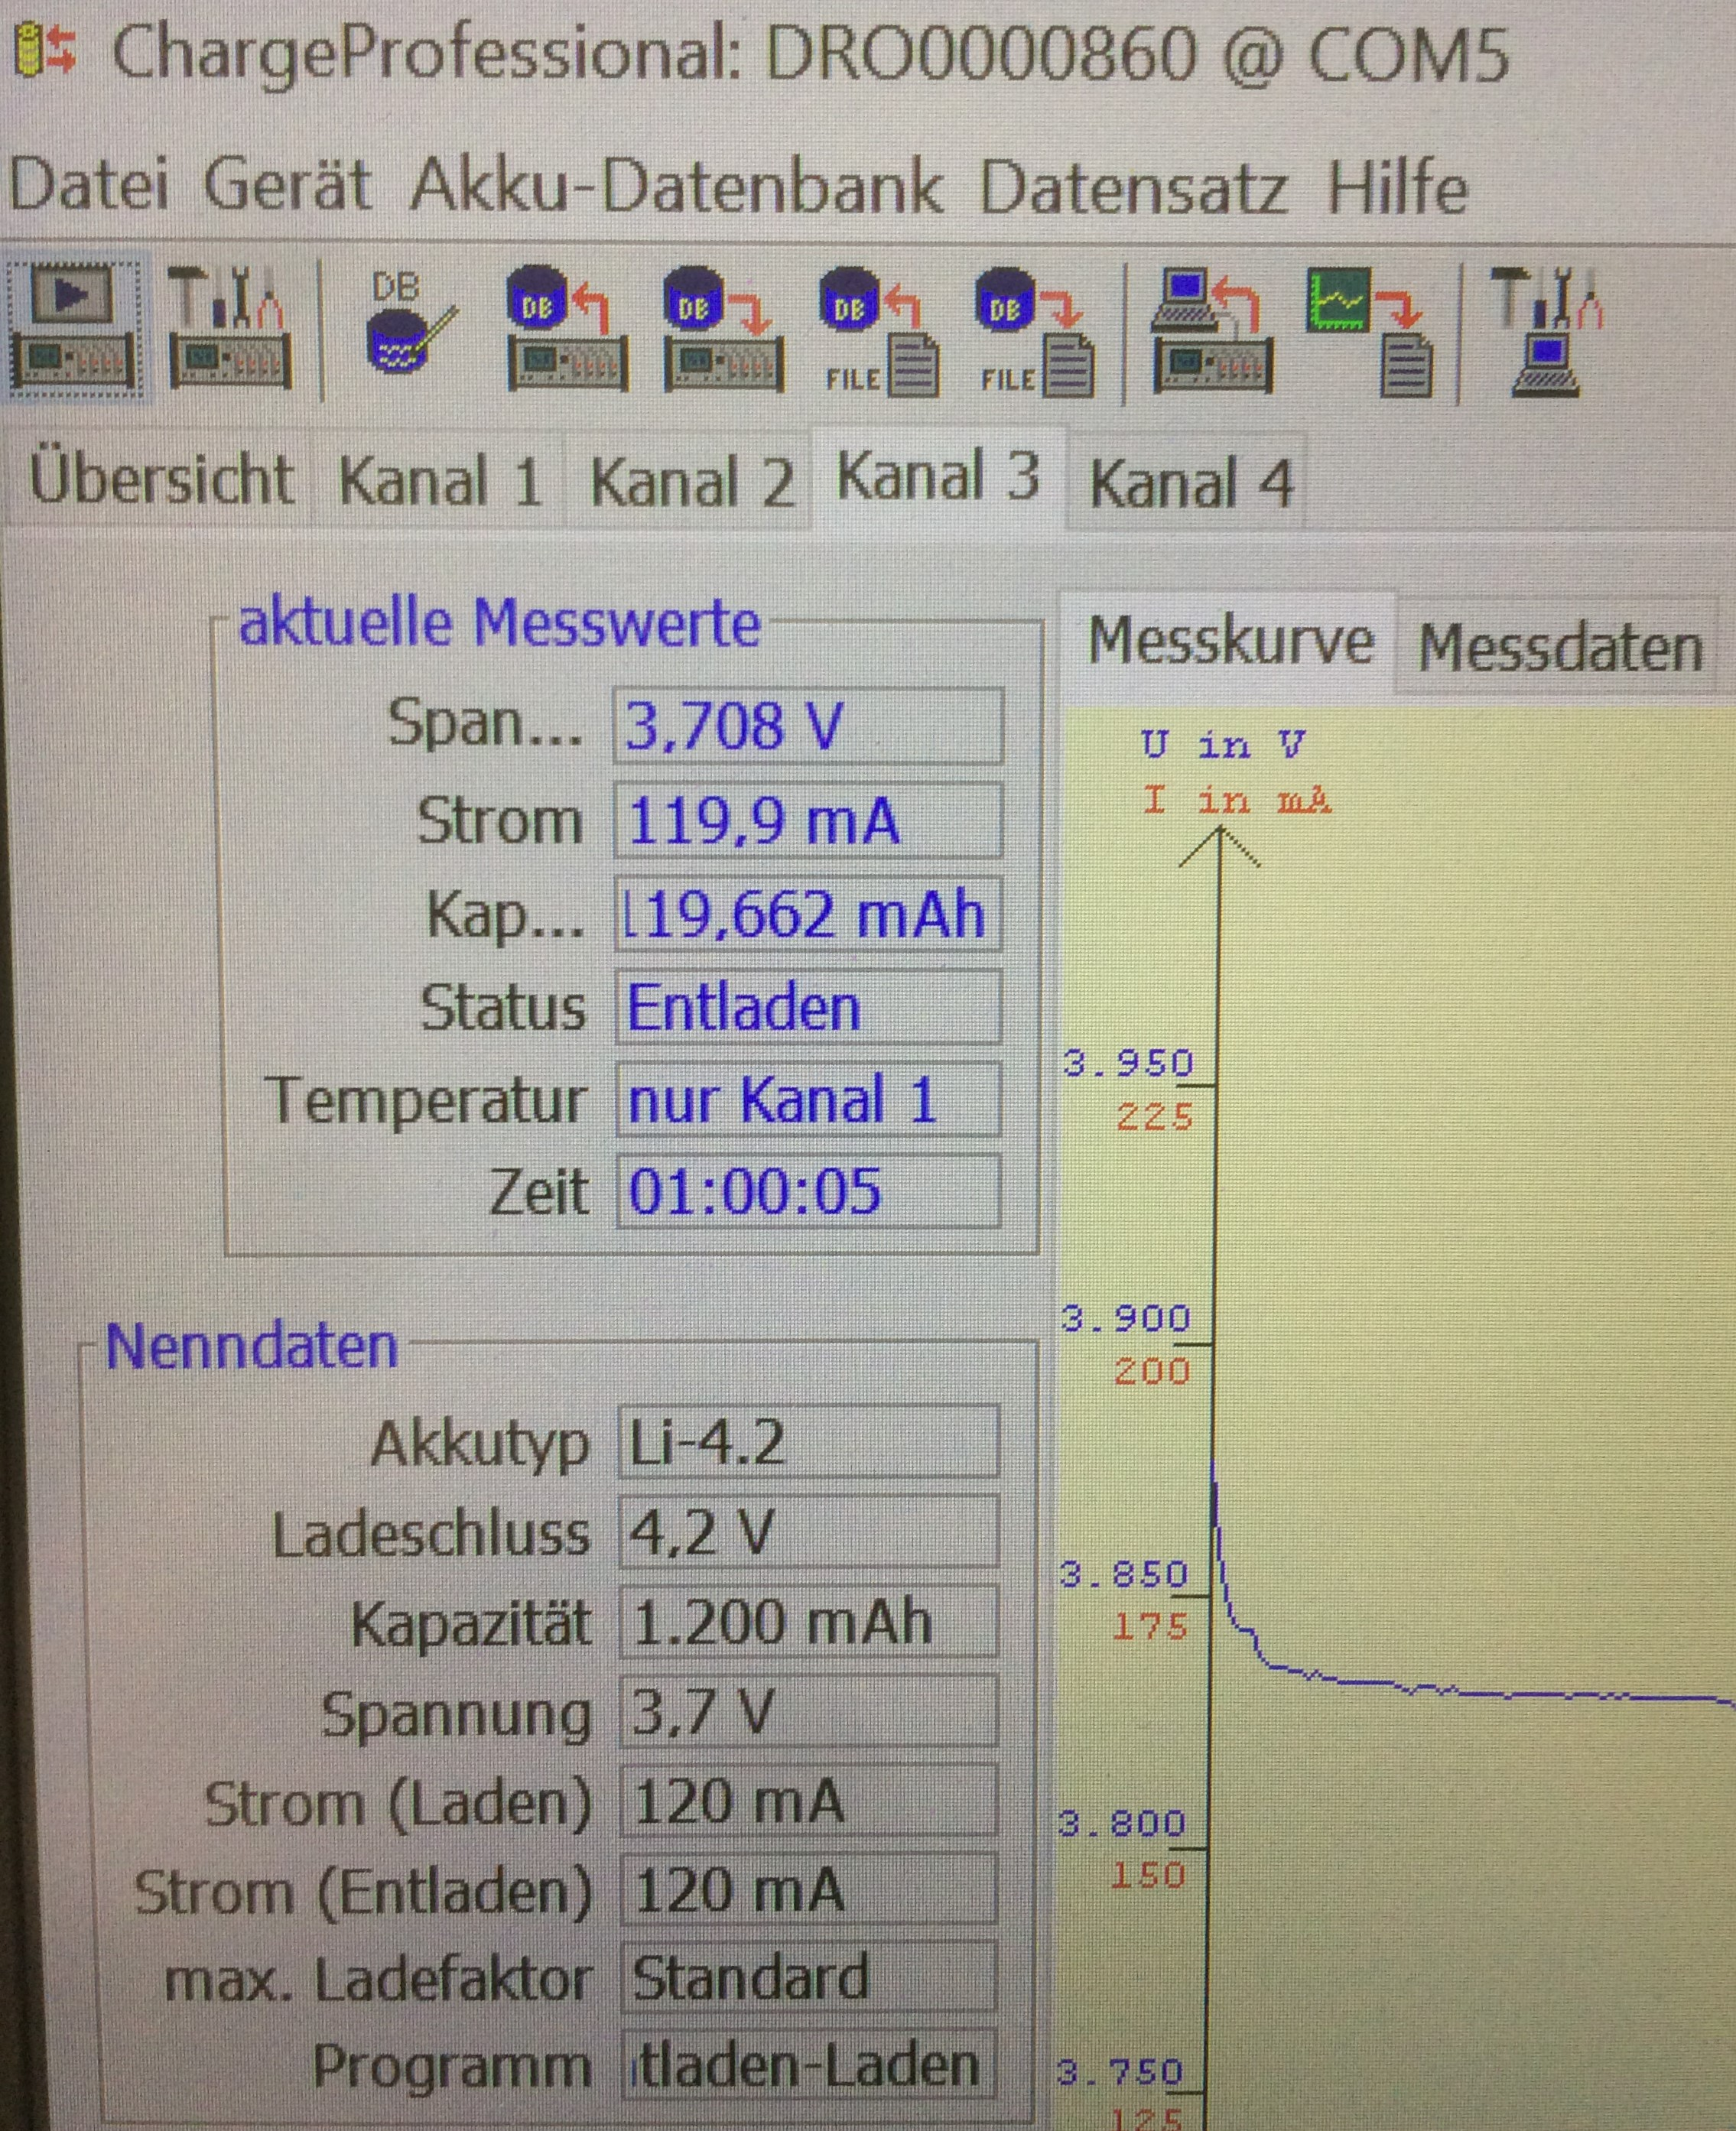
\includegraphics[width=5.5cm]{Bilder/ChargeProfessional.JPG}
	 \caption{Bildschirmausschnitt der PC-Software zum Akkutestgerät}
	 \label{fig:ChargeProfessional}
\end{figure}
%%%%%%

Der Akku wurde mit unterschiedlichen Entlade-/Ladezyklen getestet. Für den geprüften Akku von Emmerich konnte bei Entladung mit einer anfänglichen Spannung von $4.1V$ eine Kapazität von $827mAh$ gemessen werden bis der Tiefentladeschutz die Entladung bei $2.7V$ gestoppt hat. Bis zum Erreichen der internen Versorgungsspannung von $3.3V$, die im Betrieb des Dojos gehalten werden muss, konnte eine Kapazität von immerhin noch $788mAh$ festgestellt werden. Mit diesen gemessenen Werten stimmt der Akku mit den Datenblattwerten überein. Eine Entladekurve wird in Abbildung \ref{fig:Entladekurve} gezeigt.\\

%%%%%%
\begin{figure}[htp]
	\centering
	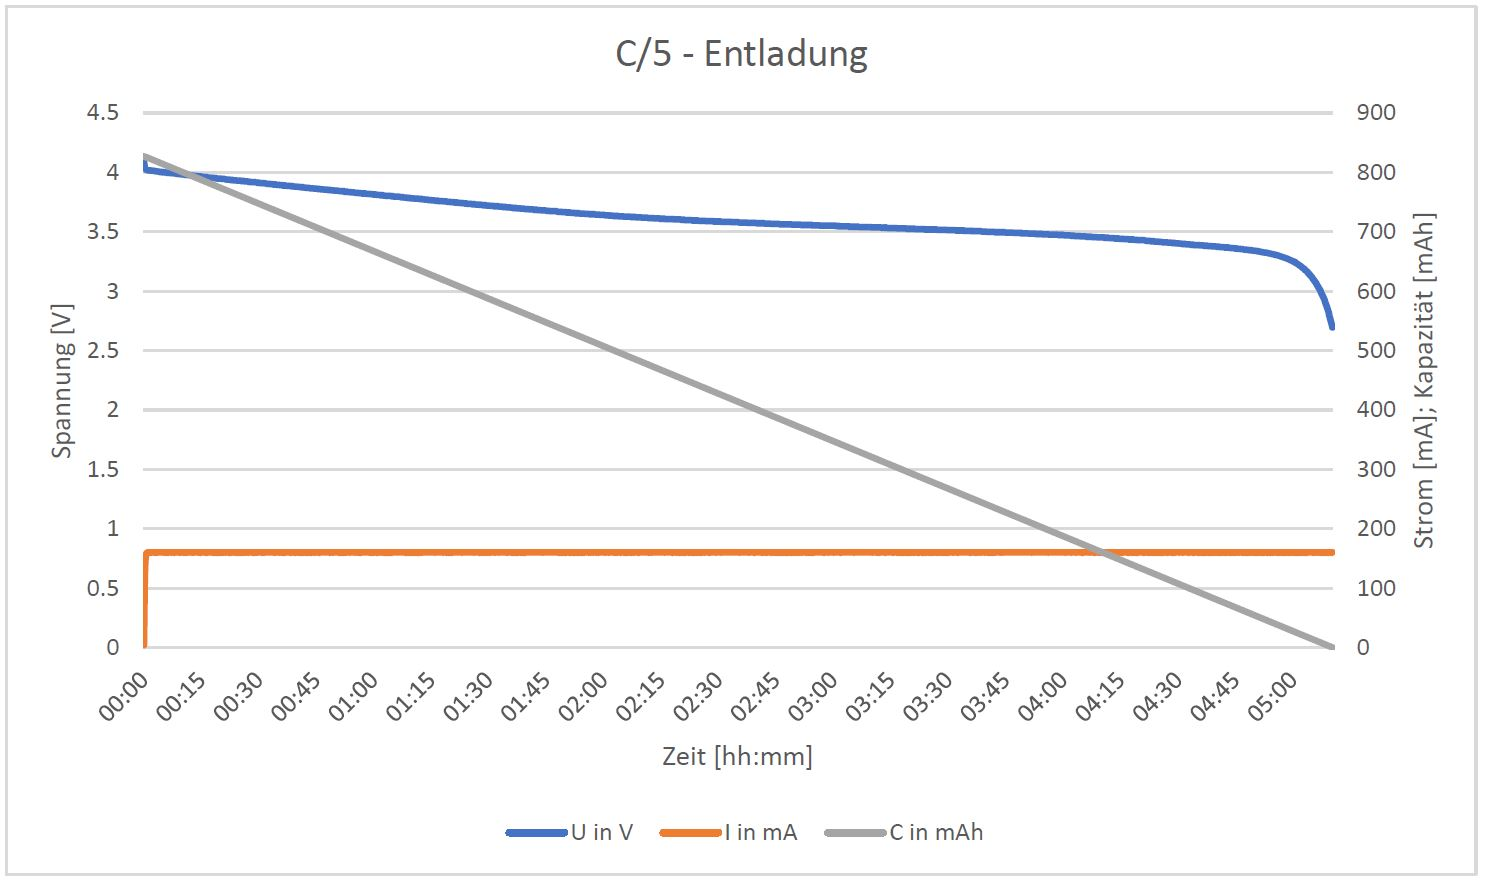
\includegraphics[width=15cm]{Bilder/Entladekurve.JPG}
	 \caption{Entladekurve des Emmerich-Akkus bei konstantem Entladestrom}
	 \label{fig:Entladekurve}
\end{figure}
%%%%%%

Neben der Kapazitätsüberprüfung des Akkus wurden auch die anfänglich nach Datenblattangaben berechneten Strombedarfswerte verifiziert. Dazu wurden am Prototyp Strommessungen durchgeführt. Die Strommessung direkt am Akku hat ergeben, dass im Standby-Betrieb, wenn also der Knochenschallgeber nicht in Betrieb ist, ein Strom von $35mA$ fliesst. Ist der Knochenschallgeber in Betrieb, steigt der Stromfluss auf $130mA$. Beim Test wurde eine Sprachdatei abgespielt, die Lautstärke war eher am oberen Limit.\\

Die Berechnung mit den gemessenen Werten zeigt, dass die angestrebten Ziele mit dem Prototyp erreicht werden. Die Speicherkapazität des eingesetzten Akkus reicht für einen Betrieb während zehn Stunden, bei einer aktiven Nutzung während $40\%$ der Zeit, also vier Stunden reine Abspielzeit und sechs Stunden Standby-Betrieb.\\

Des Weiteren wurde das Ladeverhalten des Akkus, wenn er am Prototyp angeschlossen ist, überprüft. Nach dem Einstecken des USB-Kabels fliesst während den ersten zehn Sekunden ein Strom von $330mA$, danach erhöhte sich der Stromfluss bei der Versuchsmessung auf $406mA$. Die Anhebung des Ladestromes erfolgt in einem Schritt und nicht allmählich über die Zeit. Anschliessend reduzierte sich der Strom über die Zeit allmählich, da bereits die spannungsbedingte Strombegrenzung erreicht war. Als Gegenstück diente ein USB 3.0-Anschluss eines Laptops.\\


%%%%%%
\begin{figure}[htp]
	\centering
	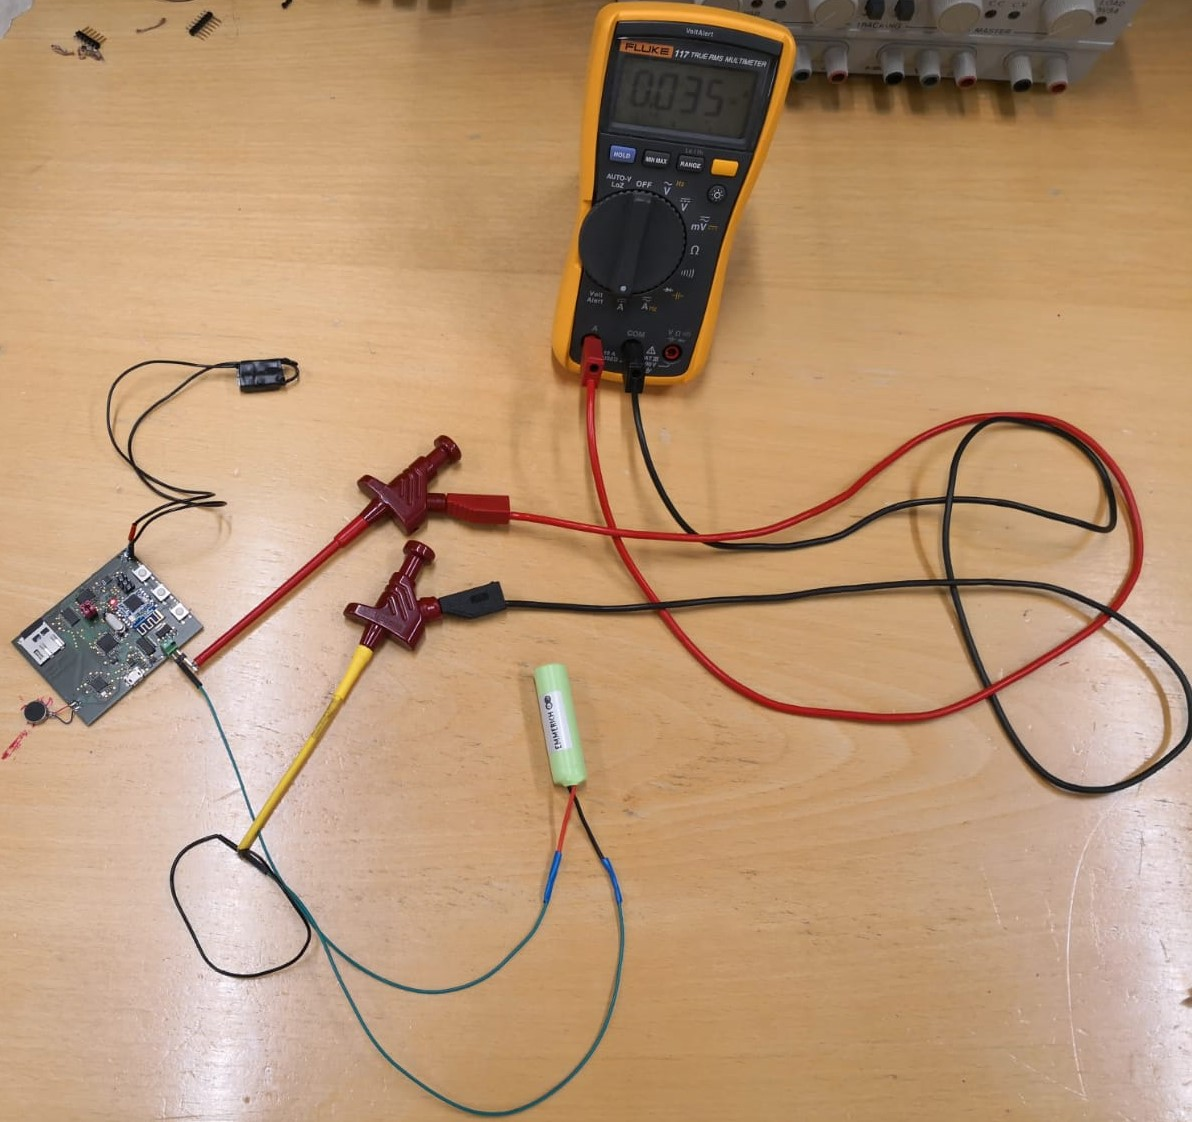
\includegraphics[width=10cm]{Bilder/StrommessungAkku.JPG}
	 \caption{Anordnung für die Strommessung am Akku}
	 \label{fig:StrommessungAkku}
\end{figure}
%%%%%%


\section{Fazit und Empfehlungen für das weitere Vorgehen}

Wie mit den vorhergehenden Berechnungen gezeigt, konnte das Ziel erreicht werden, Energiereserven für einen ganzen Betriebstag im Dojo zu speichern. Allerdings wurde ein Akku verwendet, der mit dem LI14500-Standard etwas zu gross ist für das vorgegebene Gehäusedesign. Falls bei der Weiterentwicklung der vorliegenden Dojo-Elektronik weitere Einsparungen im Energiebedarf realisiert werden können, kann der Wechsel auf einen Akku der nächstkleineren Bauart geprüft werden. Der gewählte Akku stellte sich als gut und den Herstellerangaben entsprechend heraus. Für eine Serienproduktion des Dojos ist der Preis des Akkus von Emmerich mit CHF 13.95 auf jeden Fall zu hoch. Der Preis müsste durch Verhandlung und Mengenrabatte mindestens um die Hälfte reduziert werden. Allenfalls ist in Erwägung zu ziehen, ob eine reine Speicherzelle verwendet werden soll, die keine integrierte Schutzelektronik besitzt, denn in der im Rahmen dieses Projektes entwickelten Elektronik ist ebenfalls eine Schutzbeschaltung enthalten. Die Überladeschutzschaltung hat sich im Praxistest bewährt. Sie lässt den angeschlossenen Akku mit einer zuverlässigen Ladekurve aufladen. Auch die Schaltung für das Bereitstellen der Versorgungsspannung hat sich bewährt und die Elektronik mit einer konstanten Spannung versorgt. 
